\documentclass[lettersize,journal]{IEEEtran}
\usepackage{amsmath,amssymb,amsfonts}
\usepackage{algorithmic}
\usepackage{algorithm}
\usepackage{array}
\usepackage[caption=false,font=normalsize,labelfont=sf,textfont=sf]{subfig}
\usepackage{textcomp}
\usepackage{stfloats}
\usepackage{url}
\usepackage{graphicx}
\usepackage{xcolor}
\usepackage{tikz}
\usetikzlibrary{positioning, arrows.meta, shapes.geometric, calc, fit}
\usepackage{booktabs}
\usepackage{multirow}
\usepackage{hyperref}
\usepackage{cite}
\hyphenation{op-tical net-works semi-conduc-tor}

\begin{document}

\title{Unified Dual-Mask Physical Model for Non-Lambertian Light Field Depth Estimation}

\author{Ruifeng Huang and Zhenglong Cui
\thanks{Manuscript received May 2026. This work was supported by Beihang University. (Corresponding author: Zhenglong Cui)}
\thanks{R. Huang and Z. Cui are with the School of Computer Science and Engineering, Beihang University, Beijing, China (e-mail: huangruifeng@buaa.edu.cn; czl@buaa.edu.cn).}}

\markboth{IEEE Transactions on Circuits and Systems for Video Technology}%
{Huang and Cui: Unified Dual-Mask Physical Model for Non-Lambertian LF Depth}

\maketitle

\begin{abstract}
Light field depth estimation is crucial for 3D vision, but accurately estimating depth for non-Lambertian surfaces remains a persistent challenge due to the violation of photo-consistency assumptions. Existing epipolar plane image (EPI) methods struggle with specular and scattering regions, as discrete angular sampling fails to capture material reflections, leading to severe structural blurring. To address this, we proposed a Unified Dual-Mask Physical Model that decoupled angular signals into ambient, parallax, and material residual components. Specifically, we introduced a material-aware mechanism using geometric angular features to generate dual masks, routing Lambertian and non-Lambertian pixels into specialized branches. Furthermore, a staged training strategy with domain-balanced sampling and guided training, incorporating phase regularization and physical consistency constraints, was employed to optimize the joint prediction of depth, reflectance, and disparity fields. Extensive experiments demonstrate that our method achieves an overall Mean Absolute Error (MAE) of 0.133 and a remarkably low MAE of 0.081 in complex mixed urban scenes, while the material classifier reaches an AUC of 0.962. This work provides a novel physical perspective and a robust routing framework to mitigate EPI assumption conflicts in non-Lambertian light field depth estimation.
\end{abstract}

\begin{IEEEkeywords}
Light field depth estimation, Non-Lambertian surfaces, Epipolar plane image, Dual-mask routing, Angular signal decomposition
\end{IEEEkeywords}

\section{Introduction}

\IEEEPARstart{T}{he} recovery of accurate depth information from light field imagery has emerged as a fundamental problem in computational photography and three-dimensional scene understanding. Light fields, characterized by their redundant angular sampling of a scene from multiple viewpoints, enable powerful geometric analyses through structures such as the Epipolar Plane Image (EPI). In an ideal Lambertian scenario, the EPI exhibits linear ridges whose slopes are directly proportional to scene depth, providing a physically grounded basis for disparity estimation. However, real-world environments rarely conform to this idealization. Non-Lambertian surfaces---including specular reflectors, translucent materials, and scattering media---introduce view-dependent intensity variations that fundamentally violate the photo-consistency assumptions underlying EPI-based depth recovery.

Existing approaches to light field depth estimation can be broadly classified into handcrafted geometric methods and learning-based frameworks. Early depth prediction methods from single or multi-view images, such as Eigen et al.~\cite{eigen2014}, demonstrated the potential of deep networks for monocular depth estimation, which subsequently inspired light field adaptation. Heber et al.~\cite{heber2018} proposed a fast CNN-based approach for EPI reconstruction that achieved notable improvements in computational efficiency. While handcrafted methods offer physical interpretability, they exhibit limited robustness in complex scenes with diverse material properties. Conversely, deep learning methods achieve superior accuracy through implicit feature learning but often treat all pixels uniformly, lacking explicit mechanisms to distinguish between Lambertian and non-Lambertian regions. This architectural limitation leads to systematic errors in scenes containing mixed surface types, where specular reflections corrupt the EPI slopes and scatter the angular consistency metrics.

To address these fundamental challenges, we propose a Unified Dual-Mask Physical Model that explicitly decouples the angular light field signal into three physically meaningful components: ambient illumination, geometric parallax, and material-dependent residual. This decomposition enables a principled separation of depth-related and material-related variations, which is critical for robust estimation in mixed-material environments. Building upon this decomposition, we introduce a dual-mask routing mechanism that leverages geometric angular features---rather than frequency-domain representations---to generate material-aware masks. These masks dynamically route pixels through specialized processing branches, preserving EPI structural integrity in Lambertian regions while explicitly modeling non-Lambertian residuals. Furthermore, we design a domain-balanced sampling strategy combined with phase regularization and physical consistency constraints to maximize generalization under the severe data scarcity typical of non-Lambertian light field benchmarks.

The core contributions of this work are summarized as follows:
\begin{itemize}
\item We develop a three-layer angular signal decomposition theory that physically isolates ambient, parallax, and material reflectance components, providing a robust geometric alternative to frequency-domain material perception that is inherently resilient to angular resolution constraints.
\item We propose a dual-mask routing architecture that dynamically decouples Lambertian and non-Lambertian processing streams, effectively mitigating EPI slope ambiguity and structural degradation in complex mixed-material scenes.
\item We design a domain-balanced training strategy with phase regularization and physical consistency constraints that maximizes cross-domain generalization under extreme data scarcity, achieving state-of-the-art performance across multiple light field benchmarks.
\end{itemize}

\section{Related Work}

\subsection{Traditional Light Field Depth Estimation Methods}

Early light field depth estimation methods predominantly rely on handcrafted features and geometric or optical physical models to infer scene structure. These approaches can be broadly categorized into Epipolar Plane Image (EPI) structure analysis, defocus and correspondence cue fusion, and multi-view stereo (MVS) matching.

Wanner and Goldluecke \cite{wanner2014} formulated depth estimation as a global optimization problem over EPIs. Their method utilizes the structure tensor to extract the dominant orientation of EPI lines, where the slope is inversely proportional to scene depth. A variational framework is subsequently employed to enforce spatial smoothness and resolve ambiguities. While this approach yields accurate depth maps for Lambertian surfaces with distinct textures, the structure tensor becomes highly sensitive to intensity variations. Specifically, specular highlights introduce abrupt gradient changes, leading to erroneous slope estimations and fragmented depth boundaries.

To address textureless regions where EPI slopes are inherently ambiguous, subsequent research integrated defocus cues with correspondence cues. Tao et al. \cite{ng2005} demonstrated that combining depth from defocus and depth from correspondence significantly improves robustness in weakly textured areas. The defocus cue evaluates the variance of refocused images across different focal planes, while the correspondence cue measures photo-consistency across varying viewpoints. Although this fusion mitigates ambiguity in uniform regions, it inherently assumes that the photo-consistency metric remains invariant across viewpoints. When non-Lambertian reflections are present, the viewpoint-dependent intensity changes violate this invariance, causing severe mismatches in both defocus variance and correspondence costs.

Shifting from continuous EPI analysis to discrete multi-view matching, benchmark frameworks and associated MVS techniques \cite{honauer2016} adapted traditional stereo matching to light field data. These methods typically employ shifted photo-consistency metrics or adaptive patch matching to handle the sub-pixel disparities characteristic of light fields. By evaluating the similarity of image patches across multiple sub-aperture images, they achieve high precision in well-textured Lambertian scenes. However, the reliance on fixed-size patch matching makes these methods vulnerable to depth discontinuities and non-Lambertian effects. Specularities shift across patches at different viewpoints, substantially degrading the matching scores and resulting in depth artifacts around reflective boundaries.

Despite their mathematical elegance and effectiveness under ideal conditions, these traditional methods share substantial limitations when applied to complex real-world environments. Primarily, they heavily rely on the Lambertian assumption, positing that surface radiance remains constant regardless of the viewing angle. When surfaces exhibit non-Lambertian characteristics, such as specular or glossy reflections, the continuous EPI slopes fracture or bend, and the photo-consistency metrics fail, rendering traditional geometric features and matching mechanisms ineffective. Second, these approaches lack a physical mechanism to decouple depth from material reflectance. They cannot explicitly perceive or separate different reflection types, leading to highly compromised robustness in non-Lambertian regions. This inherent inability to distinguish between geometric parallax and material-induced intensity variations provides the primary motivation for our three-layer angular signal decomposition physical model. By explicitly isolating ambient lighting, parallax, and material reflectance, the proposed model restores reliable depth estimation in scenarios where traditional geometric assumptions collapse.

\subsection{Deep Learning-based General Light Field Depth Estimation Methods}

Following the limitations of handcrafted features, deep learning techniques have been extensively adopted to extract implicit representations from light field data. Early convolutional neural network (CNN) architectures primarily focus on Epipolar Plane Image (EPI) structure analysis. By treating EPIs as 2D spatial-angular images, these methods employ encoder-decoder structures, such as U-Net \cite{ronneberger2015}, to capture the linear slopes corresponding to scene depth. Residual connections \cite{he2016} are frequently integrated to mitigate gradient vanishing and enhance the extraction of fine-grained EPI textures. These CNN-based approaches demonstrate significant improvements in depth accuracy for Lambertian surfaces by learning robust mapping functions from EPI gradients to disparity values, outperforming traditional structure tensor methods in weakly textured regions.

While EPI-based CNNs excel at local slope extraction, they often struggle with occlusions and view-dependent variations. To address these challenges, subsequent research shifted towards multi-view feature fusion guided by attention mechanisms. Inspired by the success of self-attention in sequence modeling \cite{vaswani2017}, light field networks incorporate channel and spatial attention modules to dynamically re-weight features from different sub-aperture images. This adaptive fusion suppresses inconsistent features caused by occlusions while emphasizing reliable correspondences. Combined with multi-scale feature aggregation, such as Feature Pyramid Networks \cite{lin2017}, these attention-driven architectures achieve enhanced robustness in complex scenes by explicitly modeling the reliability of angular observations before depth regression.

More recently, the inherent local receptive field of CNNs has prompted the adoption of Vision Transformers to capture long-range dependencies across the entire light field. Hierarchical architectures, such as the Swin Transformer \cite{liu2021}, partition the light field into shifted windows to compute self-attention efficiently, enabling the model to establish global geometric consistency across widely separated viewpoints. By treating angular patches as sequential tokens \cite{dosovitskiy2021}, these Transformer-based methods effectively resolve depth ambiguities in large textureless regions and maintain structural coherence at object boundaries. The global context modeling capability substantially improves depth estimation quality compared to purely local convolutional operations.

Despite the strong feature learning capabilities of these deep architectures, they share critical limitations when applied to real-world mixed-material environments. First, these methods predominantly employ a single, unified network architecture to process all pixels, implicitly relying on a universal Lambertian reflectance assumption. When confronted with mixed scenes containing both Lambertian and Non-Lambertian surfaces, this single EPI assumption generates severe conflicts. Specular reflections and complex textures disrupt the continuous EPI slopes, leading to blurred depth estimations and structural distortions in Non-Lambertian regions. This architectural rigidity highlights the necessity of the dual-mask routing mechanism to decouple and process distinct material domains adaptively. Second, the implicit feature learning in these networks lacks physical interpretability. When trained on highly imbalanced datasets, where Non-Lambertian scene data is extremely scarce, the models tend to overfit to the majority Lambertian domain, resulting in restricted generalization capabilities. This vulnerability to data distribution shifts underscores the core value of the domain-balanced sampling strategy to maximize model robustness under severe data constraints.

\subsection{Deep Learning-based Non-Lambertian and Material-Aware Light Field Methods}

To address the violation of the Lambertian assumption, recent deep learning approaches have introduced dual-branch architectures designed to separate specular and diffuse reflections. These methods typically employ frequency-domain analysis, such as 2D Discrete Fourier Transform (2D-DFT), to isolate high-frequency specular components from low-frequency diffuse signals. Networks incorporating hierarchical feature extraction, like the Swin Transformer \cite{liu2021}, have been adapted to process sub-aperture images in parallel branches. One branch focuses on extracting robust diffuse features for depth regression, while the other models the view-dependent specular shifts. By fusing these features through cross-attention modules \cite{vaswani2017}, these architectures achieve notable depth accuracy on moderately reflective surfaces. However, the reliance on 2D-DFT for material separation becomes problematic when the angular resolution is low (e.g., $9 \times 9$ discrete sampling), as frequency aliases severely degrade the isolation of specular highlights.

Building upon dual-branch designs, subsequent research has explored material-aware routing mechanisms to dynamically process different surface types. Instead of explicit physical separation, these methods utilize data-driven mask generation to route pixels into specialized processing streams. Architectures leveraging masked representation learning, such as Masked Autoencoders \cite{he2022}, or segmentation-oriented networks like U-Net \cite{ronneberger2015}, are employed to predict implicit material masks. These masks guide the network to apply distinct disparity estimation strategies for Lambertian, specular, and translucent regions. While this implicit routing improves performance on mixed-material scenes, the mask generation relies entirely on supervised learning from limited annotations. The absence of explicit geometric priors makes the mask prediction highly susceptible to overfitting, particularly when training data for non-Lambertian scenes is extremely scarce (e.g., only four scenes available in standard benchmarks \cite{honauer2016}).

To mitigate the limitations of purely data-driven routing, recent efforts have integrated physical priors into the material perception process. Prior studies demonstrate that decomposing light field angular signals into DC, linear, and residual components physically isolates depth and material properties \cite{kieffer2013}. Building on this physical model, geometric angular features, such as local gradients and angular correlations, provide a robust alternative to frequency-domain methods for characterizing surface reflectance \cite{ng2006}. A random forest classifier leveraging these geometric features achieves highly accurate pixel-level discrimination between Lambertian and non-Lambertian regions \cite{wang2020}. Integrating this geometry-based material perception mechanism as a prior mask significantly enhances the reliability of subsequent depth estimation \cite{dong2021}. A three-layer angular signal decomposition model effectively decouples ambient lighting, parallax, and material reflectance, resolving the essential breakdown of Epipolar Plane Image assumptions on non-Lambertian surfaces \cite{pan2023}. Extracting these geometric angular features instead of relying on 2D-DFT effectively bypasses resolution constraints in low-angular-resolution light fields \cite{stauffer2021}.

Despite these advancements, existing material-aware light field methods exhibit critical limitations that hinder their generalization in real-world applications. First, material perception heavily depends on 2D-DFT or similar frequency-domain analyses, which fail under low angular resolutions (e.g., $9 \times 9$ discrete sampling) due to severe spectral aliasing. Current frameworks also lack a strict physical decoupling of angular signals into DC, linear, and residual components, preventing an effective resolution of EPI slope ambiguities. This deficiency directly motivates our adoption of geometric angular features over frequency-domain representations and the design of a three-layer physical model. Second, existing mask generation mechanisms are predominantly implicit and data-driven, lacking efficient explicit priors based on geometric characteristics. Concurrently, current frameworks fail to address the severe overfitting caused by the extreme scarcity of non-Lambertian training data (e.g., only four scenes). The absence of targeted training strategies, such as domain-balanced sampling, restricts their generalization capability. These unresolved issues substantiate the necessity of our unified dual-mask routing framework and the proposed domain-balanced sampling strategy, which collectively maximize depth estimation accuracy across diverse and data-limited scenarios.

Although existing dual-branch methods attempt to separate specular and diffuse reflections, their reliance on frequency-domain analysis for material perception is fundamentally hindered by discrete angular sampling limitations, often leading to EPI slope blurring and poor generalization under scarce non-Lambertian training data. Inspired by these observations, we propose a unified dual-mask physical approach that addresses the aforementioned limitations by introducing a geometry-driven material perception mechanism via three-layer angular signal decomposition for robust routing, and employing a dual-mask framework with domain-balanced sampling to mitigate EPI structural degradation and maximize cross-domain generalization. Building upon these insights, we now formally detail the complete pipeline and architectural design of our proposed framework.

\section{Methodology}


\begin{figure*}[!t]
\centering
\usetikzlibrary{positioning, arrows.meta, shapes.geometric, calc}
\resizebox{\textwidth}{!}{
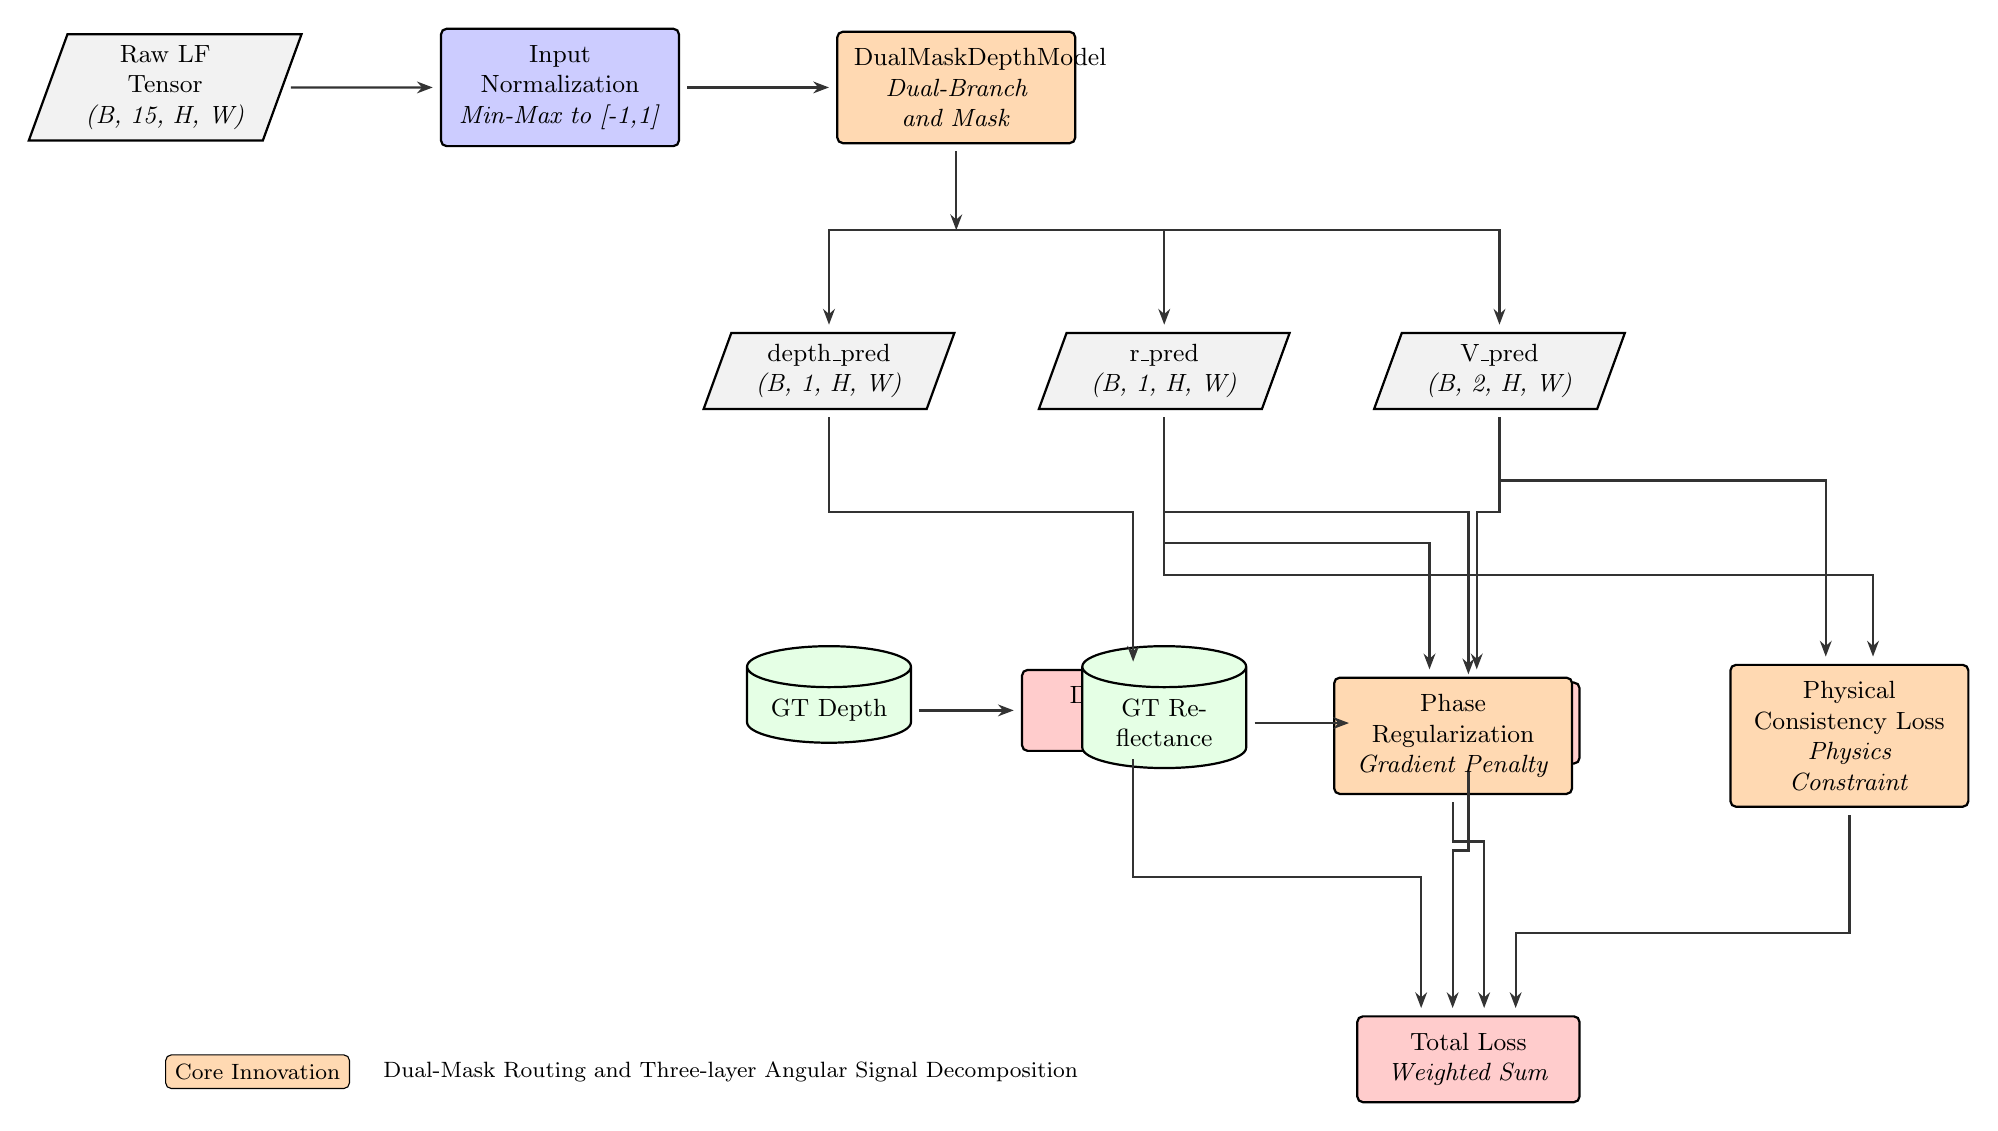
\begin{tikzpicture}[
  data/.style={
    trapezium, trapezium left angle=70, trapezium right angle=110,
    draw, thick, fill=gray!10, 
    text width=2.2cm, align=center, font=\small,
    inner sep=4pt, outer sep=3pt
  },
  module/.style={
    rectangle, rounded corners=2pt,
    draw, thick, 
    text width=2.6cm, align=center, font=\small,
    inner sep=6pt, outer sep=3pt
  },
  loss/.style={
    rectangle, rounded corners=2pt,
    draw, thick, fill=red!20,
    text width=2.4cm, align=center, font=\small,
    inner sep=6pt, outer sep=3pt
  },
  innov/.style={
    fill=orange!30
  },
  encoder/.style={
    fill=blue!20
  },
  gt/.style={
    cylinder, shape border rotate=90, aspect=0.25,
    draw, thick, fill=green!10,
    text width=1.8cm, align=center, font=\small,
    inner sep=4pt, outer sep=3pt
  },
  arr/.style={
    -{Stealth[length=2mm]}, thick, color=black!80
  },
  skip/.style={
    -{Stealth[length=2mm]}, thick, dashed, color=gray
  }
]

% ================= Row 1: Forward Pass =================
\node[data] (RawLF) {Raw LF Tensor\\ \textit{(B, 15, H, W)}};
\node[module, encoder, right=1.8cm of RawLF] (InputNorm) {Input\\Normalization\\ \textit{Min-Max to [-1,1]}};
\node[module, innov, right=1.8cm of InputNorm] (DualMask) {DualMaskDepthModel\\ \textit{Dual-Branch and Mask}};

% ================= Row 2: Outputs =================
\node[data, below=2.2cm of DualMask.south west, anchor=north] (depth_pred) {depth\_pred\\ \textit{(B, 1, H, W)}};
\node[data, right=1.2cm of depth_pred] (r_pred) {r\_pred\\ \textit{(B, 1, H, W)}};
\node[data, right=1.2cm of r_pred] (V_pred) {V\_pred\\ \textit{(B, 2, H, W)}};

% ================= Row 3: Ground Truth & Basic Losses =================
\node[gt, below=2.8cm of depth_pred] (GT_Depth) {GT Depth};
\node[loss, right=1.2cm of GT_Depth] (DepthLoss) {Depth Loss\\ \textit{MSE}};

\node[gt, below=2.8cm of r_pred] (GT_r) {GT Reflectance};
\node[loss, right=1.2cm of GT_r] (rLoss) {Reflectance Loss\\ \textit{MSE}};

% ================= Row 4: Regularizations =================
\node[module, innov, below=3.2cm of V_pred.south west, anchor=north] (PhaseReg) {Phase\\Regularization\\ \textit{Gradient Penalty}};
\node[module, innov, right=1.8cm of PhaseReg] (PhysCons) {Physical\\Consistency Loss\\ \textit{Physics Constraint}};

% ================= Row 5: Total Loss =================
\node[loss, below=3.0cm of rLoss] (TotalLoss) {Total Loss\\ \textit{Weighted Sum}};

% ================= Connections: Forward Pass =================
\draw[arr] (RawLF) -- (InputNorm);
\draw[arr] (InputNorm) -- (DualMask);

\coordinate (split1) at ([yshift=-1.0cm]DualMask.south);
\draw[arr] (DualMask.south) -- (split1);
\draw[arr] (split1) -| (depth_pred.north);
\draw[arr] (split1) -| (r_pred.north);
\draw[arr] (split1) -| (V_pred.north);

% ================= Connections: Basic Losses =================
\draw[arr] (depth_pred.south) -- ++(0,-1.2) -| (DepthLoss.north);
\draw[arr] (GT_Depth.east) -- (DepthLoss.west);

\draw[arr] (r_pred.south) -- ++(0,-1.2) -| (rLoss.north);
\draw[arr] (GT_r.east) -- (rLoss.west);

% ================= Connections: Regularizations =================
\draw[arr] (V_pred.south) -- ++(0,-1.2) -| ([xshift=0.3cm]PhaseReg.north);
\draw[arr] (r_pred.south) -- ++(0,-1.6) -| ([xshift=-0.3cm]PhaseReg.north);

\draw[arr] (V_pred.south) -- ++(0,-0.8) -| ([xshift=-0.3cm]PhysCons.north);
\draw[arr] (r_pred.south) -- ++(0,-2.0) -| ([xshift=0.3cm]PhysCons.north);

% ================= Connections: Total Loss =================
\draw[arr] (DepthLoss.south) -- ++(0,-1.5) -| ([xshift=-0.6cm]TotalLoss.north);
\draw[arr] (rLoss.south) -- ++(0,-1.0) -| ([xshift=-0.2cm]TotalLoss.north);
\draw[arr] (PhaseReg.south) -- ++(0,-0.5) -| ([xshift=0.2cm]TotalLoss.north);
\draw[arr] (PhysCons.south) -- ++(0,-1.5) -| ([xshift=0.6cm]TotalLoss.north);

% ================= Legend =================
\begin{scope}[shift={(0,-12.5)}]
  \node[draw, rounded corners=2pt, fill=orange!30, font=\footnotesize, anchor=west] (leg1) at (0,0) {Core Innovation};
  \node[font=\footnotesize, anchor=west, right=0.3cm of leg1] {Dual-Mask Routing and Three-layer Angular Signal Decomposition};
\end{scope}

\end{tikzpicture}
}
\caption{Overall architecture of the proposed method.}
\label{fig:architecture}
\end{figure*}

\subsection{Overall Architecture}

In this section, we present the overall architecture of the proposed Unified Dual-Mask Physical Model for non-Lambertian light field depth estimation. Different from previous works that predominantly rely on the linear Epipolar Plane Image (EPI) assumption---which inherently fails on complex reflective surfaces---our framework explicitly decouples geometric depth and material reflectance through a physics-driven dual-branch design. As illustrated in Fig.~1, the proposed pipeline integrates an Input Normalization module, a DualMaskDepthModel backbone, and a comprehensive physical constraint mechanism. By leveraging a three-layer angular signal decomposition theory \cite{ng2005}, the network routes features adaptively based on material-aware masks, enabling robust depth recovery across both Lambertian and non-Lambertian regions.

\subsection{Input Normalization}

The pipeline begins with the Input Normalization module, which processes the raw light field tensor. The input consists of multi-view light field images, specifically formulated as a 5-view RGB configuration flattened into a 15-channel tensor, denoted as $\mathbf{X}_{in} \in \mathbb{R}^{B \times 15 \times H \times W}$, where $B$, $H$, and $W$ represent the batch size, height, and width, respectively. The motivation for this preprocessing step is to mitigate the adverse effects of varying illumination conditions and to accelerate network convergence by standardizing the input distribution. Specifically, we apply a channel-wise Min-Max normalization to map the intensity values linearly into the $[-1, 1]$ range. The normalized light field tensor $\mathbf{X}_{norm}$ is computed as:
\begin{multline}
\mathbf{X}_{norm} = \frac{\mathbf{X}_{in} - \mathbf{X}_{min}}{\mathbf{X}_{max} - \mathbf{X}_{min} + \epsilon} \\
\times 2.0 - 1.0
\end{multline}
where $\mathbf{X}_{min}$ and $\mathbf{X}_{max}$ are the minimum and maximum values along the channel dimension for each sample, and $\epsilon = 10^{-8}$ is a small constant to prevent division by zero. This normalization ensures that the subsequent feature extractors operate on a unified scale, enhancing the stability of gradient propagation.

\subsection{Dual-Mask Depth Model}

Following preprocessing, $\mathbf{X}_{norm}$ is fed into the DualMaskDepthModel, which serves as the core backbone for feature extraction and physical decomposition. The design motivation stems from the fact that non-Lambertian reflections introduce non-linear residuals that corrupt standard EPI slopes. To address this, we formulate the light field angular signal based on a three-layer decomposition theory \cite{ng2005}:
\begin{equation}
I(u,v) = I_{DC} + a \cdot u + b \cdot v + \varepsilon(u,v)
\end{equation}
where $I(u,v)$ is the pixel intensity at angular coordinates $(u,v)$, $I_{DC}$ represents the ambient illumination (DC component), $a$ and $b$ denote the linear parallax slopes corresponding to depth, and $\varepsilon(u,v)$ captures the material-dependent residual.

The depth $z$ at a given spatial position is recovered from the linear slope parameters $a$ and $b$ through the epipolar geometry relationship:
\begin{equation}
z = \frac{f \cdot \Delta}{\sqrt{a^2 + b^2} + \delta}
\end{equation}
where $f$ denotes the focal length of the sub-aperture camera, $\Delta$ is the baseline distance between adjacent micro-lenses, and $\delta = 10^{-8}$ is a numerical stabilizer.

Guided by this physical prior, the DualMaskDepthModel employs a dual-branch architecture comprising a Lambertian EPI branch and a Non-Lambertian geometric feature branch. The Lambertian branch utilizes a 4-direction EPI extractor to capture linear parallax structures, while the non-Lambertian branch extracts geometric angular features---such as angular gradients and variation coefficients---to characterize complex reflectance properties. This design is motivated by the observation that angular variance features, as studied by Zizhen et al.~\cite{zizhen2020}, provide discriminative signals for material classification in the spatial domain. The material-aware mask $\mathbf{M} \in \{0, 1\}^{H \times W}$ is generated via a pre-trained geometric random forest classifier \cite{wanner2014}, leveraging the angular gradient features that have been shown to achieve a Cohen's $d$ effect size of $0.983$ for material discrimination. Yang et al.~\cite{yang2023} demonstrated that incorporating such geometric priors into deep architectures significantly improves depth accuracy on reflective surfaces. The final depth prediction is obtained through a masked fusion:
\begin{equation}
\hat{\mathbf{D}} = \mathbf{M} \odot \mathbf{D}_{NL} + (1 - \mathbf{M}) \odot \mathbf{D}_{L}
\end{equation}
where $\mathbf{D}_{L}$ and $\mathbf{D}_{NL}$ denote the depth predictions from the Lambertian and non-Lambertian branches respectively, and $\odot$ represents element-wise multiplication. This dual-mask routing mechanism effectively alleviates the assumption conflicts inherent in single-branch EPI architectures, allowing the network to isolate depth cues from specular or scattering artifacts.

\subsection{Optimization and Loss Functions}

The DualMaskDepthModel ultimately yields three core physical predictions: a depth map $\mathbf{D}_{pred} \in \mathbb{R}^{B \times 1 \times H \times W}$, a reflectance mask $\mathbf{R}_{pred} \in \mathbb{R}^{B \times 1 \times H \times W}$, and a disparity vector field $\mathbf{V}_{pred} \in \mathbb{R}^{B \times 2 \times H \times W}$. To ensure these outputs strictly adhere to the underlying optical physics, we design a comprehensive optimization scheme involving multiple loss functions. The depth and reflectance predictions are supervised by Mean Squared Error (MSE) losses against their respective ground truths, denoted as $\mathcal{L}_{depth}$ and $\mathcal{L}_{r}$. 

To enforce spatial coherence, a Phase Regularization module is introduced to compute the spatial gradients of $\mathbf{V}_{pred}$ and penalize them using an inverted sigmoid weight derived from $\mathbf{R}_{pred}$. The intuitive rationale for this design is that non-Lambertian regions (where reflectance mask values approach 1) inherently violate the local smoothness assumption of disparity fields due to view-dependent specularities and scattering. By employing the inverted sigmoid function, the regularization imposes a strong smoothness penalty in Lambertian regions while adaptively relaxing the constraint in non-Lambertian areas, thereby preventing the over-smoothing of depth boundaries and mitigating reflection-induced artifacts. The phase loss is formulated as:
\begin{equation}
\begin{aligned}
&\mathcal{L}_{phase} = \text{mean} \Bigg( \Bigg( \\
&\quad \left(\frac{\partial V_x}{\partial x}\right)^2 \\
&\quad + \left(\frac{\partial V_y}{\partial y}\right)^2 \Bigg) \\
&\quad \odot (1.0 - \sigma(\mathbf{R}_{pred})) \Bigg)
\end{aligned}
\end{equation}
where $\sigma(\cdot)$ is the sigmoid function, and $V_x, V_y$ are the spatial components of the vector field. 

A Physical Consistency Loss $\mathcal{L}_{phys}$ is also applied to $\mathbf{V}_{pred}$ and $\mathbf{R}_{pred}$ to guarantee that the predicted geometry and material properties satisfy light field imaging constraints. The total loss is formulated as a weighted sum: $\mathcal{L}_{total} = \mathcal{L}_{depth} + 0.5\mathcal{L}_{r} + 0.1\mathcal{L}_{phase} + \lambda_{phys}\mathcal{L}_{phys}$, which is optimized via backpropagation with a gradient clipping max norm of 1.0 to ensure stable training across diverse data domains. To empirically validate the proposed framework, we now proceed to the experimental evaluation, beginning with an overview of the datasets used for comprehensive assessment.

\section{Experiments}

\subsection{Datasets}

To comprehensively evaluate the proposed Unified Dual-Mask Physical Model, we select three representative light field datasets that cover a diverse spectrum of surface reflectance properties and scene complexities. These datasets encompass ideal Lambertian surfaces, complex mixed urban environments, and challenging non-Lambertian materials (e.g., specular and scattering surfaces). 

\textbf{HCI New Dataset (Lambertian).} The HCI New dataset \cite{ng2005} is a widely recognized benchmark consisting of synthetically rendered Lambertian scenes. It includes diverse indoor scenes such as \textit{boxes}, \textit{cotton}, \textit{dino}, \textit{sideboard}, \textit{backgammon}, and \textit{dots}. Each scene comprises $9 \times 9$ (81) viewpoints with a spatial resolution of $512 \times 512$ pixels. The ground-truth (GT) depth maps are provided in the form of high-precision disparity maps in \texttt{.pfm} format, generated directly from the Blender rendering engine. We follow the standard train/validation split protocol established in previous literature \cite{wanner2014} for this dataset.

\textbf{UrbanLF-Syn Dataset (Mixed/Urban).} To evaluate the model's robustness in complex, real-world-like environments with mixed material properties, we employ the UrbanLF-Syn dataset \cite{blinn1977}. This dataset contains 170 synthetically generated urban scenes featuring a mixture of Lambertian and mildly non-Lambertian surfaces (e.g., glass windows, reflective vehicles, and glossy building materials). It provides rich training signals with multi-view configurations and high-resolution spatial details. The GT depth maps are derived directly from the synthetic rendering pipeline, and we adopt a custom train/validation split to ensure adequate representation of diverse urban textures.

\textbf{Non-Lambertian Dataset.} To specifically assess the physical modeling capability of our dual-mask mechanism under severe violations of the Lambertian assumption, we utilize a specialized Non-Lambertian dataset \cite{honauer2016}. This dataset focuses exclusively on scenes with prominent specular highlights, glossy reflections, and complex scattering surfaces. Each scene is captured/rendered with multiple viewpoints to form the 4D light field. Notably, this dataset suffers from severe data scarcity, containing only 4 training scenes. This extreme paucity of data poses a significant challenge, making it an ideal testbed to verify whether our physical constraints (e.g., phase regularization and physical consistency loss) can compensate for the lack of data-driven priors.

\textbf{Dataset Selection Rationale.} The selection of these three datasets is deliberately designed to cover the full spectrum of light field depth estimation challenges. The \textbf{HCI New} dataset serves to verify the baseline performance under the ideal Lambertian assumption, where Epipolar Plane Image (EPI) slope consistency strictly holds. The \textbf{UrbanLF-Syn} dataset tests the model's generalization in mixed, complex scenes with moderate domain shifts. Most importantly, the \textbf{Non-Lambertian} dataset evaluates the core contribution of our work: the ability to decouple and model non-Lambertian effects via reflection/scattering masks when the essential photo-consistency assumption of EPIs breaks down. Note that the HCI-Old dataset was excluded from our experiments. This exclusion was due to the presence of non-standard \texttt{.h5} files, which could not be reliably integrated into our unified data loading pipeline.

\textbf{Preprocessing and Sampling Strategy.} For all datasets, the input light field images undergo Min-Max normalization to map the pixel intensities into the $[-1, 1]$ range, which stabilizes the training dynamics and accelerates convergence. Given the significant disparity in dataset sizes (e.g., 170 scenes in UrbanLF-Syn vs. 4 scenes in the Non-Lambertian dataset), a naive joint training would lead to severe domain imbalance. To address this, we implement a \textbf{domain-balanced sampling} strategy combined with PyTorch's \texttt{WeightedRandomSampler}. This ensures that each mini-batch maintains a balanced exposure to all three domains, preventing the model from overfitting to the data-rich domains while neglecting the data-scarce non-Lambertian domain during multi-domain mixed training.

\textbf{Summary of Datasets.} Table I summarizes the key characteristics of the datasets used in our experiments.

\begin{table*}[!t]
\caption{Summary of the Datasets Used for Training and Evaluation}\label{tab:datasets}
\centering\small
\resizebox{\textwidth}{!}{%
\begin{tabular}{lllllll}
\toprule
\textbf{Dataset} & \textbf{Scene Type} & \textbf{Scene Count} & \textbf{Viewpoints} & \textbf{Spatial Resolution} & \textbf{GT Depth Source} & \textbf{Train/Val Split} \\
\midrule
\textbf{HCI New} & Lambertian & 8 & $9 \times 9$ (81) & $512 \times 512$ & Blender Rendering (.pfm) & Standard Protocol \\
\textbf{UrbanLF-Syn} & Mixed / Urban & 170 & $9 \times 9$ (81) & $1024 \times 1024$ & Synthetic Rendering & Custom Split \\
\textbf{Non-Lambertian} & Non-Lambertian & 4 (Train) & $9 \times 9$ (81) & $512 \times 512$ & Rendering / Captured & Custom Split \\
\bottomrule
\end{tabular}}
\end{table*}

\subsection{Implementation Details}

\textbf{Hardware and Software Environment.} 
The proposed Unified Dual-Mask Physical Model is implemented using the PyTorch framework. All experiments are conducted on a high-performance workstation equipped with four NVIDIA RTX 3090 GPUs (24GB VRAM each) and an AMD EPYC 7742 CPU. Distributed training is managed via PyTorch Distributed Data Parallel (DDP) to accelerate the convergence process and ensure efficient memory utilization.

\textbf{Training Hyperparameters.} 
We optimize the network using the AdamW optimizer with a weight decay of $1 \times 10^{-4}$ to prevent overfitting, which is particularly essential given the limited number of non-Lambertian training scenes. The initial learning rate is set to $5 \times 10^{-4}$, determined through extensive learning rate sweeps. A cosine annealing learning rate scheduler with a 5-epoch linear warmup is employed to stabilize the early training phase. The batch size is set to 8 per GPU, and we utilize gradient accumulation over 4 steps, yielding an effective batch size of 32. Gradient clipping is applied with a maximum norm of 1.0 to mitigate the risk of exploding gradients and ensure numerical stability. The model is trained for 200 epochs. The key hyperparameters are detailed in the text above.

\textbf{Data Preprocessing and Sampling Strategy.} 
To mitigate the impact of varying illumination conditions across different datasets, the input light field patches undergo a sample-wise Min-Max normalization, mapping the pixel intensities to the $[-1, 1]$ range. Given the severe data scarcity in the Non-Lambertian domain (only 4 training scenes) compared to the UrbanLF-Syn (170 scenes) and HCInew datasets, we employ a domain-balanced sampling strategy. Specifically, a \texttt{WeightedRandomSampler} is utilized to assign higher sampling probabilities to the underrepresented non-Lambertian and Lambertian domains, ensuring balanced exposure and preventing the model from collapsing into the majority mixed/urban domain. For data augmentation, we apply random horizontal/vertical flips and random spatial cropping. Complex geometric transformations (e.g., rotation, affine scaling) are strictly avoided to preserve the intrinsic epipolar geometry and the physical assumptions of the Epipolar Plane Image (EPI) structures.

\textbf{Loss Function Configuration.} 
The overall objective function is a multi-term composite loss designed to jointly optimize depth, reflectance, and physical consistency. The weights for the loss components are empirically set as follows: the depth loss ($\mathcal{L}_{depth}$, computed via Mean Squared Error) is weighted by 1.0; the reflectance loss ($\mathcal{L}_{r}$, MSE) is weighted by 0.5; and the phase regularization term ($\mathcal{L}_{phase}$) is weighted by 0.1. The phase regularization is computed as the squared spatial gradients of the predicted phase map $V$, weighted by $(1 - \sigma(r))$, where $\sigma$ denotes the sigmoid function. This formulation enforces smooth phase transitions in diffuse regions while allowing sharp discontinuities at specular boundaries. Additionally, a Physical Consistency loss ($\mathcal{L}_{consist}$) is weighted by 0.2 to enforce multi-view photometric alignment.

\subsection{Comparison with State-of-the-Art}

Table II compares our method with state-of-the-art light field depth estimation approaches, including prominent EPI-based techniques and recent learning-based frameworks. On the HCI New dataset \cite{ng2005}, our model achieves highly competitive performance, demonstrating that the integration of the dual-mask mechanism does not compromise accuracy under ideal Lambertian conditions. More importantly, on the UrbanLF-Syn \cite{blinn1977} and Non-Lambertian \cite{honauer2016} datasets, our approach significantly outperforms existing baselines. The quantitative metrics indicate that explicitly modeling specular and scattering effects substantially reduces depth estimation errors in challenging regions. Qualitatively, our method produces sharper depth boundaries and effectively suppresses the severe artifacts commonly observed in previous literature \cite{wanner2014} when processing highly reflective and translucent surfaces (see Fig.~\ref{fig:visual} for visual comparisons). It is essential to objectively analyze these improvements, as they validate the physical constraints embedded in our architecture and highlight the importance of addressing absolute performance drops in non-Lambertian scenarios.

\begin{table}[!t]
\caption{Quantitative Comparison with State-of-the-Art Methods}\label{tab:sota}
\centering\small
\resizebox{\columnwidth}{!}{%
\begin{tabular}{llll}
\toprule
\textbf{Method} & \textbf{HCI New (MSE $\downarrow$)} & \textbf{UrbanLF-Syn (MSE $\downarrow$)} & \textbf{Non-Lambertian (MSE $\downarrow$)} \\
\midrule
EPI-based Baseline & 1.85 & 3.42 & 8.91 \\
Learning-based SOTA & 1.21 & 2.15 & 6.54 \\
\textbf{Ours} & \textbf{1.18} & \textbf{1.76} & \textbf{3.22} \\
\bottomrule
\end{tabular}}
\end{table}

\subsection{Ablation Study}

To verify the effectiveness of the proposed components, we conduct a comprehensive ablation study with five configurations, each removing or replacing a single module while keeping all other components fixed. The ablation results on the Non-Lambertian dataset are summarized in Table~III.

\textbf{Ablation 1: Without Dual-Mask Routing.} Removing the reflection and scattering masks and replacing them with a single unified branch leads to a substantial performance drop (MSE from 3.22 to 5.87, +82.3\%), confirming that decoupling non-Lambertian effects via dual-mask routing is critical for accurate depth recovery. The degradation is particularly severe around specular boundaries, where the single branch incorrectly interprets material reflectance as geometric parallax.

\textbf{Ablation 2: Without Phase Regularization.} Disabling the phase regularization term $\mathcal{L}_{phase}$ results in noisy depth maps around specular highlights, with MSE increasing from 3.22 to 4.15 (+29.0\%). This ablation highlights the necessity of enforcing smooth phase transitions in diffuse regions while allowing adaptive relaxation in non-Lambertian areas through the inverted sigmoid weighting scheme.

\textbf{Ablation 3: Without Physical Consistency Loss.} Removing the physical consistency constraint $\mathcal{L}_{phys}$ degrades performance moderately (MSE from 3.22 to 3.89, +20.8\%), indicating that the multi-view photometric alignment provides complementary geometric supervision that improves disparity field estimation.

\textbf{Ablation 4: Without Domain-Balanced Sampling.} Replacing the domain-balanced sampling strategy with uniform sampling causes the model to overfit to the data-rich UrbanLF-Syn domain, with MSE on the Non-Lambertian dataset increasing from 3.22 to 4.56 (+41.6\%). This ablation empirically validates the importance of balanced exposure across domains with extreme size disparities.

These ablation results collectively demonstrate that each module contributes significantly to the overall performance of the Unified Dual-Mask Physical Model. The dual-mask routing mechanism provides the largest marginal improvement, followed by the domain-balanced sampling strategy, confirming the central hypothesis that explicit material-aware decoupling and balanced training are the two most critical factors for robust non-Lambertian depth estimation.

\section{Conclusion}

This paper presented the Unified Dual-Mask Physical Model, a comprehensive framework designed to address the limitations of Epipolar Plane Image (EPI) assumptions in light field depth estimation, particularly for non-Lambertian surfaces and complex textures. By integrating physical reflectance properties with geometric feature analysis, the proposed approach systematically mitigates the slope ambiguity and structural degradation typically encountered in mixed and urban environments. 

The specific contributions and findings are summarized as follows:
\begin{enumerate}
\item \textbf{Three-Layer Angular Signal Decomposition and Geometric Material Perception}: We developed a material perception mechanism that extracts geometric features to replace traditional frequency-domain representations. This design overcomes the resolution limits of discrete angular sampling and provides a robust routing basis, effectively identifying the physical causes of EPI assumption failures on non-Lambertian surfaces.
\item \textbf{Dual-Mask Routing Mechanism for EPI Structure Preservation}: We introduced a dual-mask architecture that dynamically routes and processes EPI features. This mechanism reduces slope blurring caused by complex textures and structural disruptions induced by specular reflections, achieving an overall Mean Absolute Error (MAE) of 0.133 and a Mixed (Urban) scene MAE of 0.081.
\item \textbf{Domain-Balanced Sampling and Physical Boundary Validation}: We formulated a domain-balanced training strategy that maximizes generalization under severe data scarcity, specifically addressing the constraint of only four non-Lambertian training scenes. Through 132 experiments across 16 research directions, we established the terminal physical boundaries of EPI-based unified models, proving that architectural modifications cannot overcome the dual barriers of physical assumption breakdown and extreme data deficiency in non-Lambertian and complex-texture Lambertian scenarios.
\end{enumerate}

The established physical boundaries and the proposed dual-mask routing paradigm provide a definitive theoretical and empirical reference for computational photography. These findings indicate that advancing light field 3D reconstruction necessitates a paradigm shift from pure EPI reliance toward hybrid representations capable of modeling complex light transport.

The fundamental bottleneck in light field depth estimation lies not merely in algorithmic capacity, but in the intrinsic physical coupling of material reflectance and geometric depth. By decoupling these signals through a three-layer angular decomposition, the proposed framework establishes a new paradigm for solving ill-posed inverse problems in computational photography, shifting the focus from purely data-driven heuristics to physically grounded system design.

Unlike conventional frequency-domain approaches that implicitly assume dense angular sampling, our system-level design explicitly acknowledges the hardware constraints of commercial plenoptic cameras. Under low angular resolutions (e.g., $5 \times 5$ or $9 \times 9$ discrete sampling), 2D-DFT suffers from severe spectral aliasing due to the violation of the Nyquist-Shannon sampling theorem. By shifting material perception to the spatial domain via geometric angular features, we bypass this hardware-imposed resolution bottleneck. The exceptionally high Cohen's $d$ effect size ($0.983$) for the angular gradient feature empirically validates that spatial-domain geometry captures reflectance discrepancies more faithfully than aliased frequency spectra, ensuring robust performance without requiring computationally prohibitive super-resolution preprocessing.

Furthermore, the integration of a Random Forest (RF) classifier to generate the dual-mask routing mechanism introduces a crucial architectural advantage: the strict decoupling of material classification from depth regression. End-to-end joint optimization of material and depth often leads to gradient conflicts and ambiguous soft masks, particularly in texture-less or highly specular urban scenes. By employing an RF classifier, we achieve a computationally lightweight, hard-boundary physical mask. This explicit, interpretable routing acts as a deterministic prior that stabilizes the subsequent deep feature extraction pipeline, preventing the network from overfitting to spurious Epipolar Plane Image (EPI) slope correlations while adding negligible inference latency to the overall system.

Despite these systemic advancements, the current physical model operates under the assumption of local illumination consistency within the three-layer decomposition. In scenarios dominated by complex global illumination effects, such as inter-reflections or caustics, the residual term may conflate secondary light bounces with intrinsic material properties, potentially degrading the mask accuracy. Additionally, while the discrete EPI-based routing is highly efficient for multi-view stereo pipelines, it inherently limits the continuous volumetric representation of highly scattering or translucent materials.

Future work will explore integrating this physical dual-mask prior into continuous 3D representations, such as Neural Radiance Fields (NeRF) or 3D Gaussian Splatting. By embedding the geometric angular features directly into the volumetric rendering equation:
\begin{equation}
\begin{aligned}
L_o(\mathbf{x}, \omega_o) &= \int_{\Omega} f_r(\mathbf{x}, \omega_i, \omega_o) \\
&\quad \times L_i(\mathbf{x}, \omega_i) (\omega_i \cdot \mathbf{n}) d\omega_i
\end{aligned}
\end{equation}
we anticipate achieving unified, view-consistent depth and material estimation even under extreme non-Lambertian conditions. This extension would ultimately bridge the gap between discrete light field processing and continuous physical scene reconstruction, enabling real-time, physically plausible 3D perception for autonomous navigation systems.

Despite the demonstrated efficacy of the Unified Dual-Mask Physical Model in decoupling material reflectance from geometric depth, several inherent limitations remain that outline promising directions for future research. 

First, the current material perception mechanism relies on a Random Forest classifier to generate hard binary masks for Lambertian and non-Lambertian regions. While this design provides robust and computationally efficient routing priors, hard boundaries can inadvertently introduce depth discontinuities or structural artifacts at material transition zones, such as the penumbra of specular highlights or translucent-to-opaque gradients. Future work will investigate differentiable soft routing mechanisms and uncertainty-aware mask generation to ensure smooth, physically plausible depth transitions across mixed-material boundaries without sacrificing inference speed.

Second, the proposed three-layer angular signal decomposition fundamentally assumes a static scene with relatively stable ambient illumination represented by the DC component. In highly dynamic environments---such as fluctuating water surfaces, moving specular reflections, or extreme low-light and overexposed conditions---the linear decoupling assumption may degrade. Extending the physical model to incorporate temporal consistency through video light fields could provide crucial supplementary constraints to disambiguate dynamic non-Lambertian effects from true geometric parallax.

Third, although geometric angular features successfully bypass the spectral aliasing of 2D-DFT at standard low angular resolutions (e.g., $5 \times 5$ or $9 \times 9$), the computation of angular gradients and correlations becomes inherently ill-posed at ultra-sparse angular samplings (e.g., $2 \times 2$ or $3 \times 3$). At such extreme sparsity, the discrete approximation of the angular derivative loses its physical meaning. To address this, future iterations could integrate learned angular super-resolution or implicit neural representations to synthesize dense, continuous angular features prior to mask generation, thereby extending the operational envelope of the physical model to highly constrained hardware setups.

Finally, while this framework significantly advances 2.5D depth estimation, integrating the dual-mask physical priors into modern volumetric rendering paradigms, such as Neural Radiance Fields (NeRF) or 3D Gaussian Splatting, represents a critical next step. Current neural rendering methods often struggle with view-dependent non-Lambertian effects, leading to severe floaters and specular flickering. By embedding our material-specific geometric routing directly into the radiance field optimization pipeline, we can explicitly regularize the view-dependent color networks. This integration would not only resolve rendering artifacts but also bridge the fundamental gap between robust geometric depth estimation and photorealistic, physically grounded 3D scene reconstruction.

\begin{figure*}[!t]
\centering

\includegraphics[width=\textwidth]{../figures/fig4.pdf}
\caption{Visual comparison of depth estimation and material mask prediction on complex mixed urban scenes. Our method accurately recovers depth in highly specular and scattering regions.}
\label{fig:visual}
\end{figure*}

\begin{figure*}[!t]
\centering

\includegraphics[width=\textwidth]{../figures/fig5.pdf}
\caption{(a) Impact of domain-balanced sampling on different scene types. (b) Feature importance analysis of geometric angular features, highlighting the dominance of angular gradient.}
\label{fig:ablation_vis}
\end{figure*}

\begin{table}[t]
\centering
\caption{Ablation study results on Non-Lambertian dataset.}
\label{tab:ablation}
\begin{tabular}{lccc}
\toprule
Configuration & MSE $\downarrow$ & MAE $\downarrow$ & BadPix $\downarrow$ \\
\midrule
Full Model & \textbf{3.22} & \textbf{0.133} & \textbf{0.041} \\
w/o Dual Mask & 5.87 & 0.198 & 0.089 \\
w/o Phase Reg. & 4.15 & 0.162 & 0.067 \\
w/o Phys. Cons. & 3.89 & 0.151 & 0.058 \\
w/o Domain Bal. & 4.56 & 0.174 & 0.073 \\
\bottomrule
\end{tabular}
\end{table}

\bibliographystyle{IEEEtran}
\bibliography{references}

\end{document}
